
\section{Introduction and Background}
Integrative systems modeling builds on a larger tradition of system
dynamics modeling, a field that originated out of operations research
and industrial engineering.  System dynamics modeling is an method to
model the behavior of complex systems in terms of stocks, flows, and
feedback loops.  The intuition here is that \emph{stock variables}
quantify the amount of some material, or mass, (or population in
disease modeling) in a compartment at a particular moment in time,
while \emph{flow variables} quantify the amount of material moving
into, out of, or between compartments. The scope of applications for
system dynamics is enormous, and once you start thinking of systems in
this way it may seem that everything can be modeled as stocks and
flows.  This is true of many approaches to modeling, however.  The
scope of system dynamics modeling is vast, and the method is useful
across this vast scope. It has been applied to the study of complex
systems in economics, politics, environmental science, and a diverse
array of other fields.

Traditionally, there is a delineation separating system dynamics
modeling from statistical modeling in the following way: system
dynamics aims to develop a \emph{model of process}, while statistical
approaches focus on developing a \emph{model of data}. Models of
process attempt to explicitly represent the mechanisms behind some
system behavior (deterministically or stochastically), while models of
data often explicitly avoid requiring such mechanistic theories. The
advantage of using the system dynamics approach is that it can
incorporate structural assumptions about the system underlying the
data.  In most applications, however, the process models of system
dynamics and the data models of statistics remain separate.
Integrative systems modeling is an attempt to bring them together for
mutual benefit.

The field of system dynamics has grown out of the work of Jay Forrester, a
management professor at MIT with a background in science and
engineering, in the 1950s. Its first application was in explaining
employment cycles at the company's appliance plants [ref TK]. Managers
incorrectly assumed that cycles merely followed general, economic
cycles, but by developing a compartmental model of the system
underlying GE's appliance business, Forrester showed that the
employment cycles arose from feedback loops inherent to GE's internal
structure. This first application demonstrates a major theme in system
dynamics. In complex systems, determinants of system behavior
considered one-by-one may be insufficient to predict the behavior of
that system. The most important behavior in a complex system arises
out of interactions and feedback between processes in that system. In
the case of disease modeling, the information contained in modeling
the entire disease process of incidence, remission and mortality
can exceed the information contained in separate
analyses of each of these features of the disease epidemiology.

TK paragraph on forward simulation, which includes an simple example,
such as the growth of a population, or use of a renewable resource.

Pharmacokinetic and pharmacodynamic (PKPD) modeling, a subdiscipline
of pharmacology, developed an approach to compartmental modeling in
tandem with system dynamics modeling, largely independently.  However,
the mathematics behind the models of process are extremely
similar. The compartments in PKPD models represent organs and other
physical systems in the body, and stocks represent the quantities of
pharmacologically relevant compounds in these compartments.  The flows
model the process of the drug of interest being metabolized or
otherwise passing through the subject. Mathematically, these models
have precise parallels to the stock-and-flow models developed by
Forrester and colleagues for supply chain analysis. For instance, in
one experiment researchers used a system dynamics approach to model
glucose kinetics. They found that a three compartment model where two
compartments correspond to peripheral pools exchanging plasma at
different rates with a central pool best represented the physiology of
glucose kinetics in their test subjects (in this case, a sample of 7
sheep) [ref TK]. This particular model structure has arisen several
times in applications in pharmacokinetics. It is called the mammillary
model. In another experiment, researchers modeled the kinetics of FULL
NAME TK (EACA) in 6 human subjects. EACA is compound used to control
hemorrhage in patients with bleeding problems. The PKPD researchers
developed a multi-compartmental model, where EACA was infused in a
central compartment, distributed to fast and slow excreting peripheral
compartments, and cleared by two compartments, one representing renal
excretion of the drug, and another representing non-renal excretion
[ref TK]. In both of these examples, and in general practice in
pharmacokinetics, the compartmental model-of-process is connected to a
statistical model-of-data to go beyond forward simulation to develop
methods of statistical inference for compartmental models. This
connection is the central idea of integrative systems modeling, and
one will be developed in detail in later chapters.

There has increasing interest in applying system dynamics principles
to the modeling of health and health systems. Health systems are
particularly complex, with many actors and many feedback loops,
providing a large supply of systems modeling opportunities. The health
of a population is affected by a combination of biological, economic,
demographic, and political forces, and all of these spheres interact
in a unexpected ways. Since the 1970s, system dynamics models have
been applied to model these various forces in order to advance our
understanding of population health [refs TK]. The topics addressed
have included: disease epidemiology, substance abuse epidemiology,
patient flows in emergency care, health care capacity and delivery,
and interactions between health care and disease epidemiology. A
systems approach is often required, because isolating one part of a
public health problem and then addressing that may in fact adversely
affect other parts of the system. For instance, low tar/nicotine
cigarettes were developed to address one part of the burden of disease
caused by tobacco consumption, but consumer behavior was not taken
into account. Consumers tended to take longer, more frequent drags and
thus negated the benefit of the low tar/nicotine content [ref TK]. A
system approach would seek to simultaneously account for both the
effect of the tobacco product on the consumer and the consumer's
behavior. In the context of modeling the progression of a disease
through a population, a model that seems to describe infection
dynamics accurately may conflict with data on remission or
fatality. Only by modeling the three together can the analyst get the
most accurate and consistent estimates.

One area in which public health has a long tradition of compartmental
and system dynamics modeling is in infectious disease [ref Andersen
  and May, Heathecote, Sally Blower, others? see wikipedia
  compartmental models in epi page]. For example, the
Susceptible-Infected-Recovered compartmental model, which was discussed in
Section~\ref{TK}. This basic model has been extended in a variety of
ways in order to model increasingly more complex infectious disease
dynamics. For instance, in one study Nagelkerke and colleagues modeled
the impact of a range of interventions targeted at preventing
transmission of HIV/AIDS epidemics [ref]. They estimated impact using a
compartmental model where the population moved from an Uninfected
compartment to either treated or untreated Infected
compartments to an AIDS compartment to a Death from AIDS
compartment. 

Another example that makes an explicit connection between
epidemiological modeling and system dynamics is the recent work by
Kershenobich and colleagues, who applied a systems approach to
forecasting the prevalence of hepatitis C. They developed a
compartmental model tracking incidence, diagnosis and treatment of the
disease. For the incident population in the model, an individual moves
from an acute phase (which lasts for 6 months) to a chronic phase,
unless that individual is spontaneously cleared of the disease, is
treated and cured or dies. For the prevalent population in the model,
an individual moves from viraemic to non-viraemic, dies or gets
treated and cured. Separate models were also used to estimate the
mortality rate in different countries based on age, liver-related
deaths due to hepatitis C infection, and percent of the population
infected by infection drug users. Sensitivity analyses were conducted
by running the model for a number of input scenarios.  TK description
of what this model allowed the authors to do, and especially how hard
it would have been to do in any other way.

System dynamics has been applied not only to the study of disease
processes, but also the health system. Flaxman and colleagues
developed a stock-and-flow model to synthesize data on the
availability and distribution of insecticide treated bednets (ITNs)
and to predict the proportion of households who owned an ITN. This
analysis employed a Bayesian approach to estimate the parameters of
the compartmental model that describe the process of ITNs moving from
warehouses and other storage facilities into the household and
possibly getting discarded by the households or lost in the
distribution process.



TK connection to the references cited in this NIH RFP for systems modeling
\url{http://grants.nih.gov/grants/guide/pa-files/PAR-08-224.html}
\url{http://ajph.aphapublications.org/cgi/content/full/96/3/452}
\url{http://www.hpsig.com/images/f/f5/SD_background_for_public_health_%284.11.05%29.pdf}
\url{http://www.systemswiki.org/index.php?title=Health_System_Dynamics_References}
\url{http://www.chronicdisease.org/nacdd-initiatives/diabetes/professional-development/act-on-data/SDMResourceList.pdf}

TK review of all pubmed literature that has term system dynamics in
the keywords or something.

TK discussion of bednets model and analogy between this and population
PK approach.

\section{System dynamics model of disease in a population}
At the heart of the new generic disease model is a set of four
compartments representing my fundamental equations of population
health. The compartments represent the population susceptible to the
disease ($S$), the population with the condition ($C$), the population
dead due to other causes ($M$), and the population dead due to the
disease ($D$). The population moves between these boxes following the
arrows shown in the figure, transitioning from $S$ to $C$ with incidence
rate $i$, and from $C$ back to $S$ with remission rate $r$. The susceptible
population transitions into box $M$ with (without-condition) mortality
rate $m$, and the with-condition population transitions into box $M$ with
without-condition mortality rate $m$, and into by $D$ with ``excess
mortality rate'' $f$.

TK parallel between this fundamental model of disease and the demographer's
 basic demographic equation (aka the fundamental balancing equation)
 \url{http://books.google.com/books?id=CR-EXq4y8XAC&lpg=PA5&ots=_jJryixe4z&dq=%22basic%20demographic%20equation%22&pg=PA6#v=onepage&q=%22basic%20demographic%20equation%22&f=false}


\section{Compartmental Model}
\begin{figure}
\begin{center}
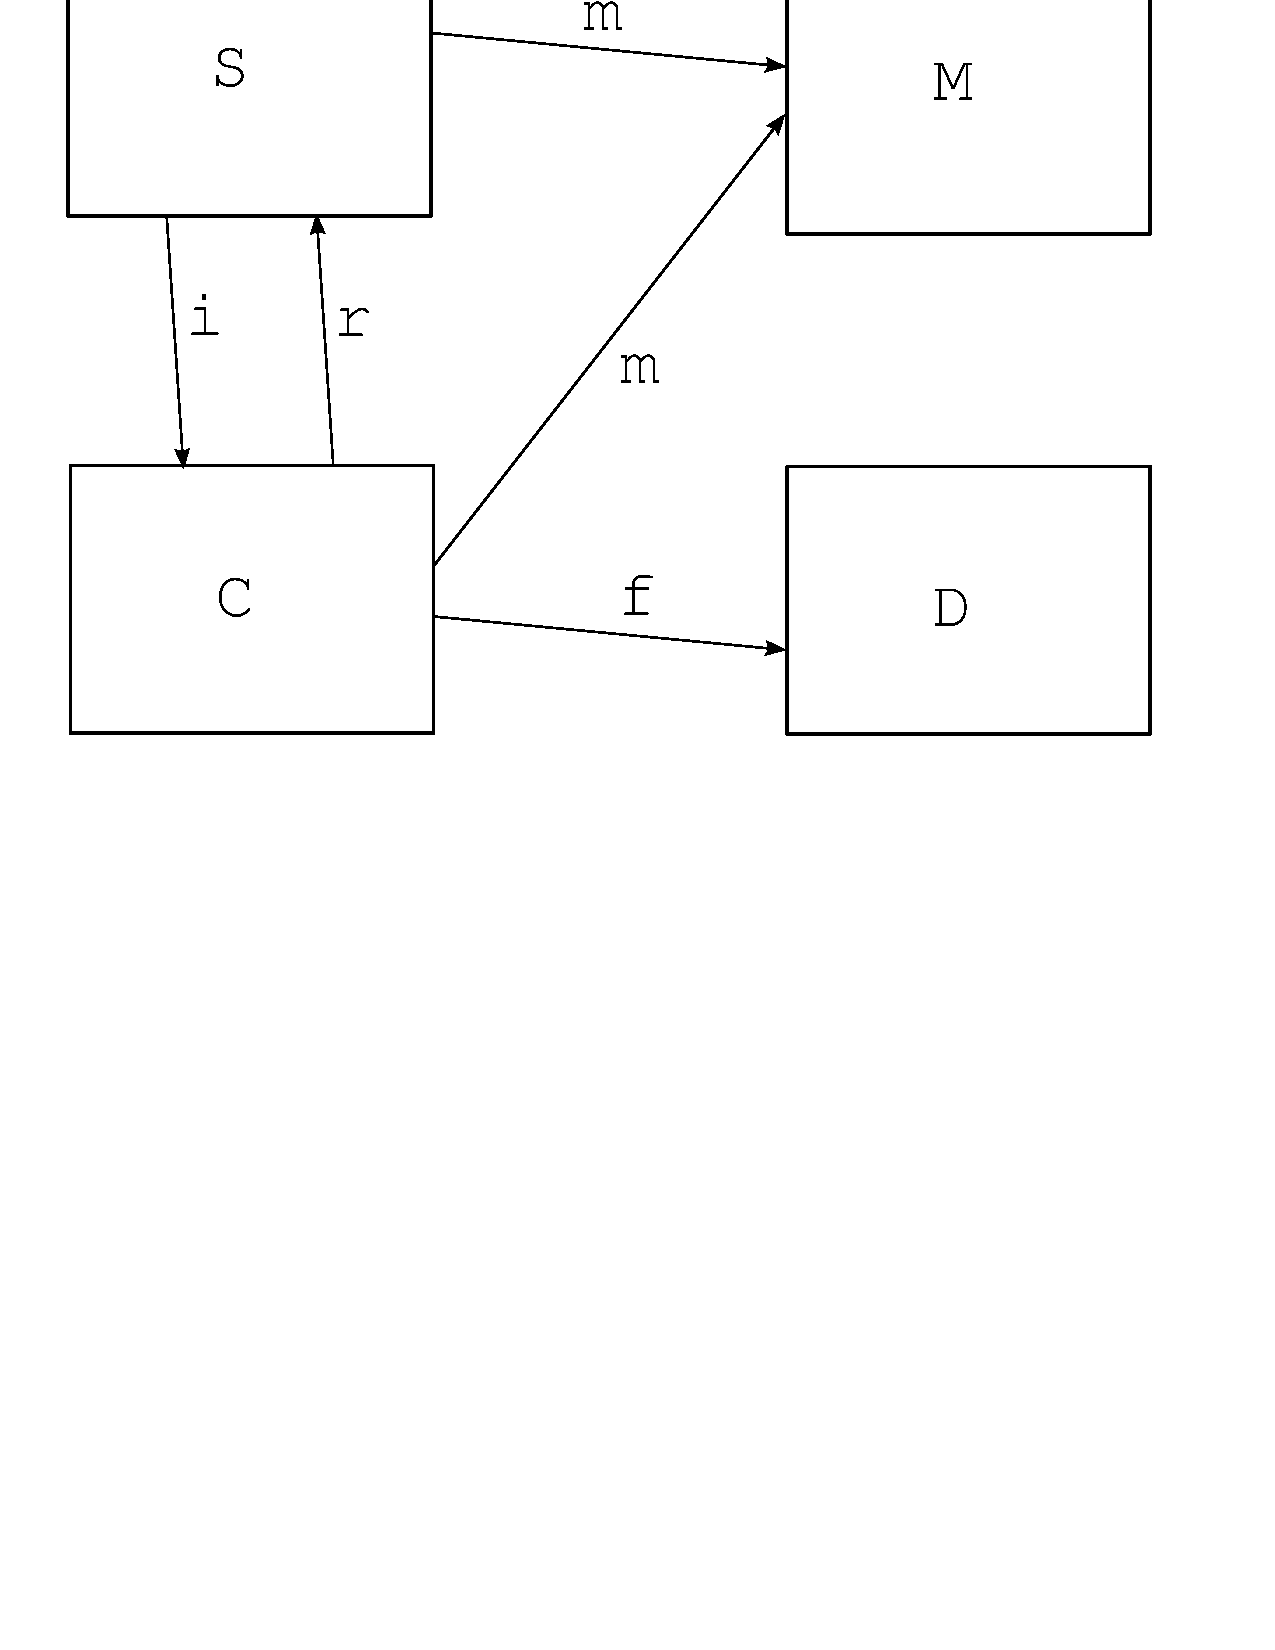
\includegraphics[width=\textwidth]{compartments.pdf}
\end{center}
\caption{TK updated caption; DisMod III uses a 4 compartment model to generate
  age-specific estimates of number without condition ($S$), number
  with condition ($C$), number of deaths not associated with the condition ($M$),
  number of deaths associated with the condition ($D$), incidence rate ($i$),
  remission rate ($r$), without-condition mortality rate ($m$), and
  excess mortality rate ($f$) (all shown in diagram); as well as
  prevalence ($p$), case duration ($X$), relative mortality risk ($RR$), all-cause mortality
  rate ($m_{all}$), and standardized mortality ratio ($SMR$).}
\label{fig:compartmental-model}
\end{figure}

TK Short discussion of what kind of epi study would be designed to
measure each of the important parts of this model. Comment that this
is not always what is available, and the bridge between what we know
and what we want to know will be developed in theory and practice in
several later sections of this book.

Conceptually, it is excess mortality $f$ that has proven hardest to
explain and to understand. This is because in most cases $f$ is a
latent variable, unobservable through most any epi study. Perhaps it
would be clearer to talk about the with-condition mortality rate,
which at least can be measured through a cohort study, and I think
will feel more familiar to the doctor or
epidemiologist. With-condition mortality is $m+f$, and the fact that
$M$ and $D$ are different boxes really is not that important when we
are doing generic disease modeling.

This 4 compartment model is really only a sketch of system dynamics
model I've used however, because it does not show age or time
information. In fact, there are large differences in disease
parameters such as incidence and prevalence as a function of age, and
it is essential for a model to take this into account.  Congenital
abnormalities all have a birth prevalence, while important diseases
such as dementia and Alzheimer's disease have much higher incidence
and prevalence at older ages. Furthermore the incidence and prevalence
of disease, as well as the remission rates and excess-mortality rates
change over time due to shifts in population, changes in prevention or
treatment, or changes in care. And the interdependence between these
factors is complex, but unignorable.  Today's 50-year-olds population
will be tomorrow's 51-year-olds, modulo migration and mortality as
least.

For these reasons, the 4 compartment model is more of a heuristic or
intuitive description of the system dynamics than a precise formal
definition.  A more accurate picture of the system dynamics model
shows the progression of the population as a function of time and age:

TK Time-age expanded version of the compartmental model above.

These figures are not up to the task of giving a full and precise
definition, however, and this is best expressed in terms of a system
of partial differential equations, describing the change in the size
of the compartments as a function of age and time. Although I have
made some simplifying assumptions for practical purposes, I believe
that it is worthwhile to start with the model that I would ideally
like to use, and then simplify it little by little so that it is
appropriately matched to the sparse data and/or the computational
resources available.

TK STOCHASTIC PDE GDM EQUATIONS, an embellishment of the following:

The full model is governed by the following system of partial
differential equations:
\begin{align*}
\frac{\partial S}{\partial (a+t)} &= -(i + m)S + rC,\\
\frac{\partial C}{\partial (a+t)} &= iS - (r + m + f)C,\\
\frac{\partial M}{\partial (a+t)} &= mS + mC,\\
\frac{\partial D}{\partial (a+t)} &= fC,
\end{align*}
where
\begin{align*}
S &= S(a,t) = \text{number without the condition of age $a$ at time $t$}\\
C &= C(a,t) = \text{number with the condition of age $a$ at
  time $t$}\\
M &= M(a,t) = \text{number dead not due to the condition (who would have been) of age $a$ at time
$t$}\\
D &= D(a,t) = \text{number dead due to the condition
  (who would have been) of age $a$ at time $t$}\\[.1in]
i &= i(a,t) = \text{incidence rate for people age $a$ at time $t$}\\
r &= r(a,t) = \text{remission rate for people age $a$ at time $t$}\\
m &= m(a,t) = \text{without-condition mortality rate for people age $a$ at
time $t$}\\
f &= f(a,t) = \text{excess mortality rate for people age $a$ at time
  $t$}
\end{align*}

\subsection{Simplifying assumptions}
\label{theory-forward_sim-compartmental_model-simplying_assumptions}

The first simplification which I have often used is to go from a
stochastic PDE to a deterministic PDE. This was done originally
because of the amount and quality of data available, as well as the
computation speed-up expected.  However, for certain data rich
settings, it may not be desirable. I suspect in the future generic
disease models will want to allow for stochastic PDEs as in the
equations above, and not be tethered by the simplifying assumptions
that I have made here. TK brief discussion of the assumptions inherent
in the deterministic model, and an investigation of how the stochastic
model could deal with these more robustly, for example deviation from
the Markovian assumption that people of age a have the same
with-condition mortality rate, regardless of whether they are a new
case or have had the condition for years. After this simplification,
the system of deterministic PDEs is the following:

\begin{align*}
\frac{\partial S}{\partial (a+t)} &= -(i + m)S + rC,\\
\frac{\partial C}{\partial (a+t)} &= iS - (r + m + f)C,\\
\frac{\partial M}{\partial (a+t)} &= mS + mC,\\
\frac{\partial D}{\partial (a+t)} &= fC,
\end{align*}

The second simplification comes from an assumption that the disease
parameters are not changing substantially with respect to time. TK
implications of simplifying assumptions on time stationarity, and
reduced equation that takes these assumptions into account.  DisMod
III follows the approach used previously, and assumes that the disease
parameters are not changing with time (i.e. the diseases is in endemic
equilibrium),
\[
\frac{\partial S}{\partial t}
=
\frac{\partial C}{\partial t}
=
\frac{\partial D}{\partial t}
=
\frac{\partial M}{\partial t}
=
\frac{\partial i}{\partial t}
=
\frac{\partial r}{\partial t}
=
\frac{\partial m}{\partial t}
=
\frac{\partial f}{\partial t}
=
0.
\]

This assumption on time derivatives is a big one, and deserves careful
assessment. In DisMod II, the default model also included the
assumption that the disease parameters did not change over time, but
an option allowed the model to incorporate assumptions of certain time
trends as well. I will return to the effects of this assumption in
section TK.

The next simplification is on the structure of the rates that dictate
the transitions between compartments (now as a function only of age).
By assuming that these rates are piecewise constant functions of age,
the system of partial differential equations has an explicit solution
for each interval on which the age is constant.

TK rewrite this lead in: Furthermore, DisMod III assumes that the rates are piecewise constant
functions of age, changing rate value only on a specified age mesh.  If
the age mesh is $\{a_0, a_1, \ldots, a_A\}$, then for any $a$ and $a'$
with $a_i \leq a, a' < a_{i+1}$,
\begin{align*}
i(a,t) &= i(a) = i(a')\\
r(a,t) &= r(a) = r(a')\\
m(a,t) &= m(a) = m(a')\\
f(a,t) &= f(a) = f(a')\\
\end{align*}

This permits me to solve the system of equations iteratively, starting
from the first interval, and proceeding interval by interval across
the entire age range. The solution for each age interval, after
assuming that TK FORMAL EQUATOIN OF ASSUMPTION takes the form of a
matrix exponential TK DISPLAY EQUATION.

These assumptions permit DisMod III to solve  explicitly for $S, C, D$
and $M$ iteratively.  The solution is conveniently expressed using the
matrix exponential:
\begin{equation}
\label{eq:ode-soln}
\begin{bmatrix}
S(a_{i+1})\\C(a_{i+1})\\M(a_{i+1})\\D(a_{i+1})
\end{bmatrix}
=
\exp\left(\begin{bmatrix}
-i(a_i)-m(a_i) & r(a_i)             & 0&0 \\
i(a_i)      & -r(a_i) -m(a_i) - f(a_i) & 0&0\\
m(a_i)      & m(a_i)             & 0&0 \\
0        & f(a_i)            & 0&0
\end{bmatrix}
(a_{i+1}-a_i)\right)
\begin{bmatrix}
S(a_i)\\C(a_i)\\M(a_i)\\D(a_i)
\end{bmatrix}
\end{equation}

There is another, related, simplification that is really more a matter
of computational convenience than mathematical simplification.  The
iterative solution to the difference equations above provides the
exact values on an age mesh $\{a_0, a_1, \ldots, a_I\}$, and this
appears in the inner-most loop of the computation, so it is a
significant time saving approximation to use linear interpolation to
fill in prevalence values between the points on the age mesh, instead
of using a more sophisticated differential equation solver to provides
a more precise solution to the system of ODEs. The effects of this
approximation can be minimized by choosing an age mesh appropriately,
and will be examined in more detail qualitatively later in the section
and quantatively in the Chapter TK on numerical algorithms.

Although the primary use of this model is for inference of model
parameters (sometimes called the ``inverse problem''), I can easily
apply it ``forwards'' to show how rates on incidence, remission, and
excess-mortality produce different prevalence curves. The next section
explores this forward simulation through a series of detailed
examples, to build up the reader's intuition around how consistency
forces interrelationships between prevalence, incidence, remission,
and mortality.


\section{Forward simulation examples}

When a generic disease model is initialized with all-cause mortality
data and nothing else, the initial values produce the following set of
consistent age patterns:

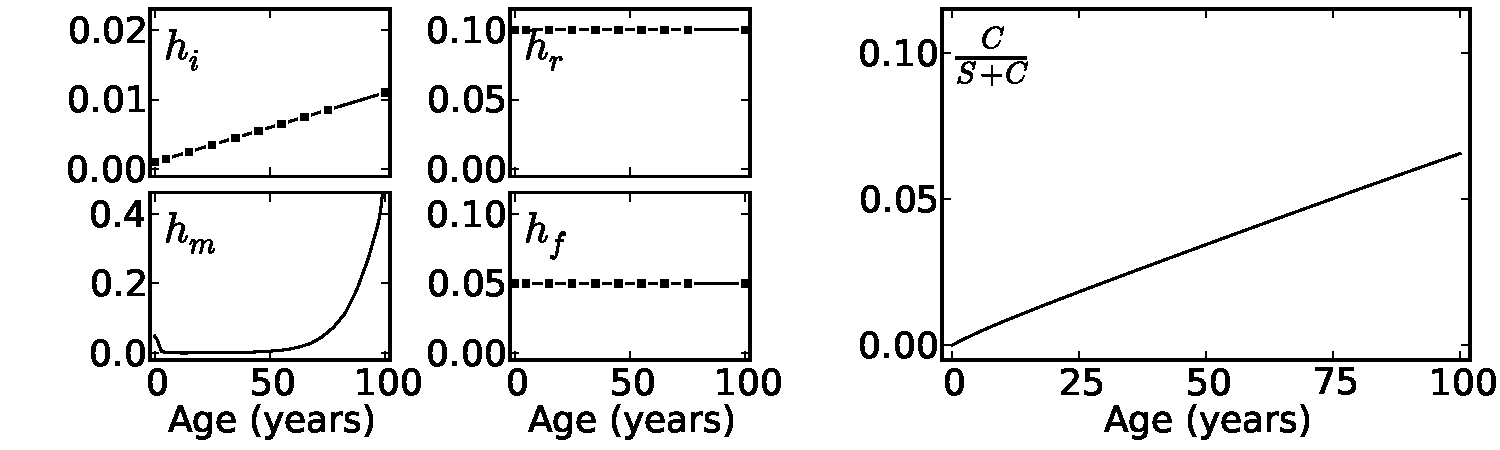
\includegraphics[width=\textwidth]{initial.png}

The next example shows that increasing the remission rate with
incidence and excess mortality unchanged (and all-cause mortality
unchanged as well) leads to a very different age pattern for
prevalence. It is also worth pointing out that since prevalence has
changed with excess mortality and all-cause mortality rates held
constant, the with-condition and background mortality rates have also
changed to maintain consistency.

\includegraphics[width=\textwidth]{more-remission.png}

By changing the incidence rate age pattern to be increasing as a
function of the square root age, I can demonstrate that very similar
prevalence rates are consistent with very different incidence and
remission rates.

\includegraphics[width=\textwidth]{increasing-incidence.png}

Although the prevalence age pattern is largely determined by the
remission, incidence, and mortality rates, the birth prevalence can
also change the shape dramatically.  Here are the results of the same
remission, incidence, and mortality rates as above, but with a birth
prevalence of 20\%.

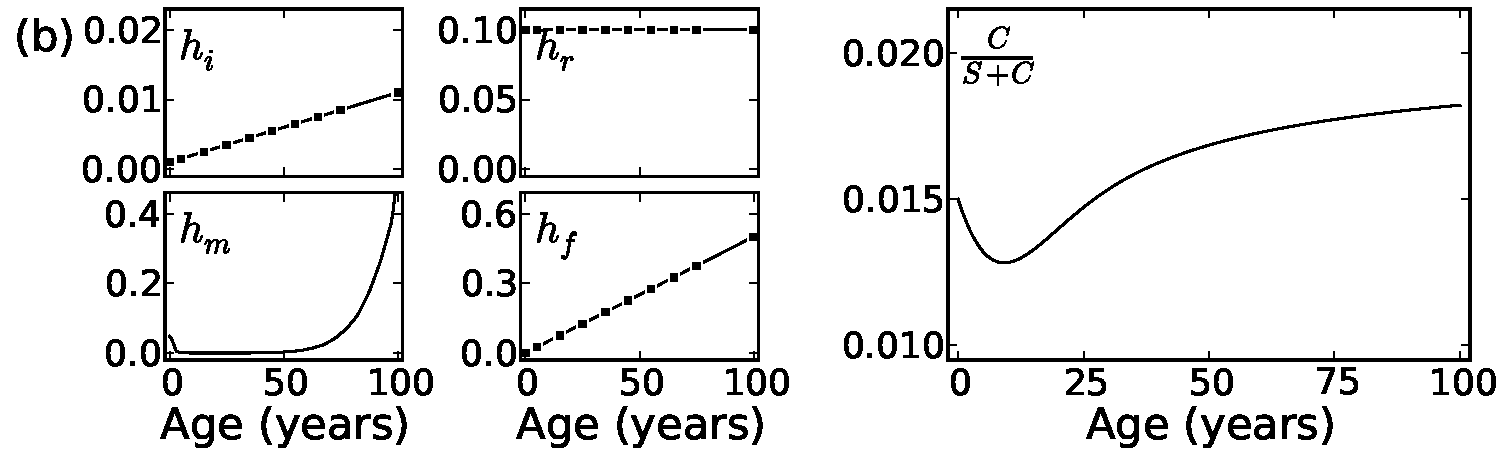
\includegraphics[width=\textwidth]{birth-prevalence.png}

An interesting, and perhaps unexpected feature of this set of
consistent rates above is that when prevalence levels start so high,
the levels remain high during the teenage years, where all-cause
mortality rates are quite low in this population (following the rates
for males in the North American High Income region in 2005), which
produces very low levels of background mortality for these age
groups. In other words, in order for the model to be consistent, it is
necessary to assume that the vast preponderance of teenage deaths are
due to this disease.

Finally, the excess mortality rate (which is the most difficult of the
rates to conceptualize, due to its unobservability) has an effect of
modulating the prevalence that is similar to the remission rate,
although not identical.  The final figure in this series shows the
results of choosing an excess mortality rate to have an age function
equal to ten times the all-cause mortality rate (which is to say a
standardized mortality rate of constant value eleven for all ages).

\includegraphics[width=\textwidth]{higher-smr.png}

The decreasing prevalence after age 65 is worthy of remarking
on. Although the incidence rate is increasing and the remission rate
remains unchanged, having a constant (albeit high) standardized
mortality ratio means that when all-cause mortality rises, the
with-condition mortality rises differentially with such magnitude that
the prevalence of the condition in older populations goes down.

To summarize, this series of figures has shown the intuitive and
less-than-intuitive way that the levels and age patterns of different
epidemiological parameters must be interrelated to satisfy the
fundamental equations of population health (when disease rates for
each age are changing negligibly slowly as a function of time).

The next series of figures continues to build familiarity with the
features of consistent disease modeling, by selecting age patterns for
certain rates based on toy models of a variety of diseases.  For
example, for a disorder like depression, for which there is primarily
incidence in early adulthood, high remission rate, and low excess
mortality, the consistency conditions produce a prevalence age pettern
that peaks at age 25: 

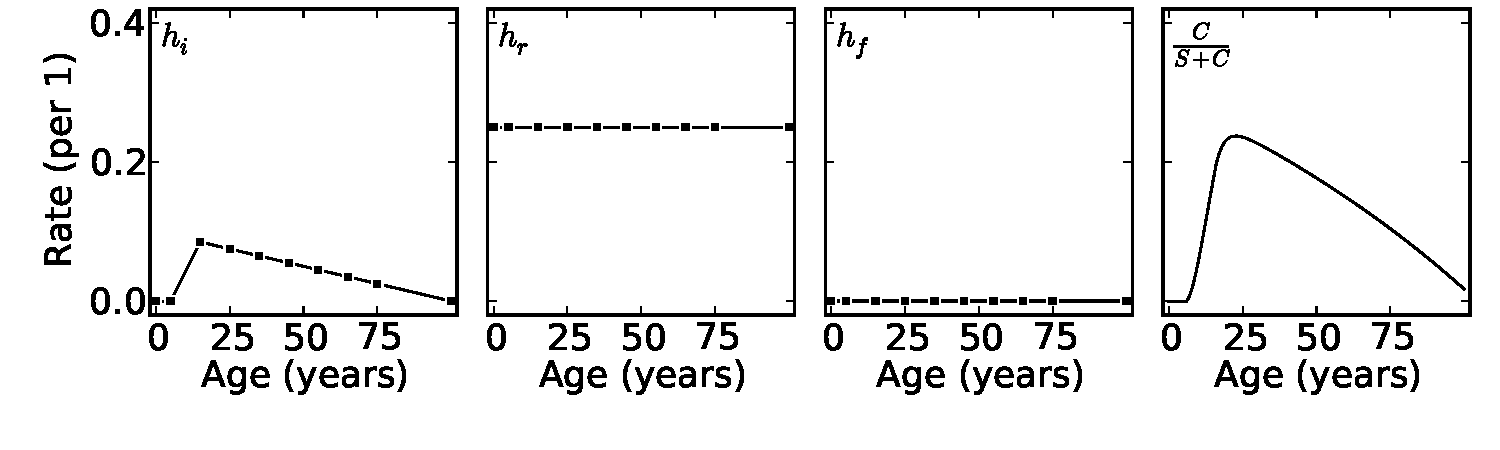
\includegraphics[width=\textwidth]{forward-sim-mental.png}

For a congenital disorder, like TK, with birth prevalence, no
incidence after birth, no remission, and substantial mortality, the
consistent prevalence age pattern is the following:

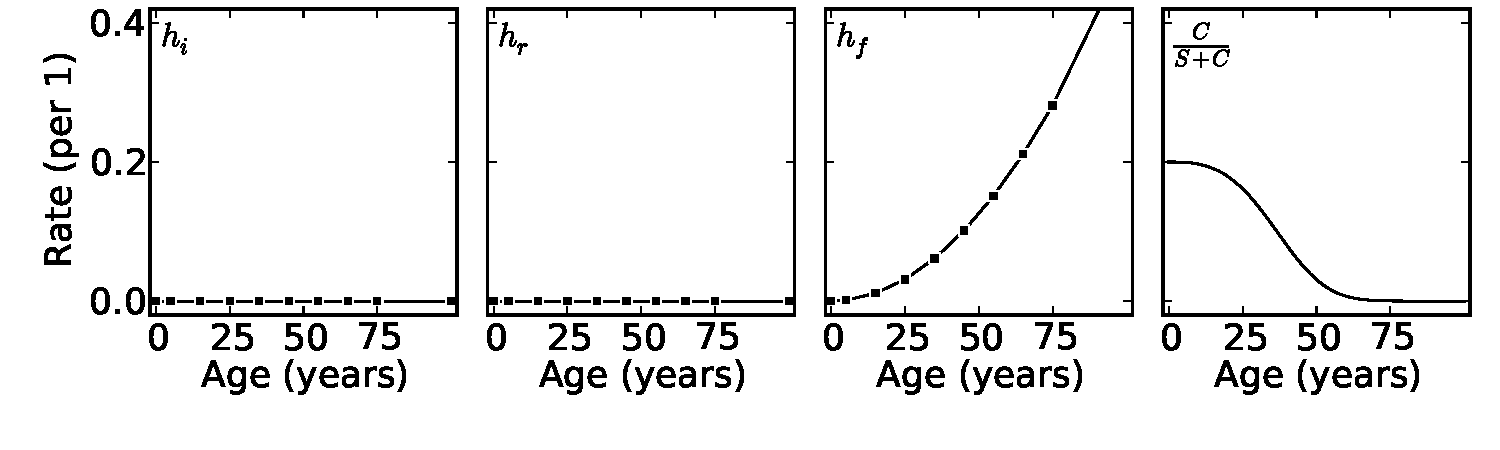
\includegraphics[width=\textwidth]{forward-sim-congenital.png}

For a disorder that affects the elderly, like TK, the consistent age
patterns for mortality, incidence, remission, and prevalence could
look like the following: 

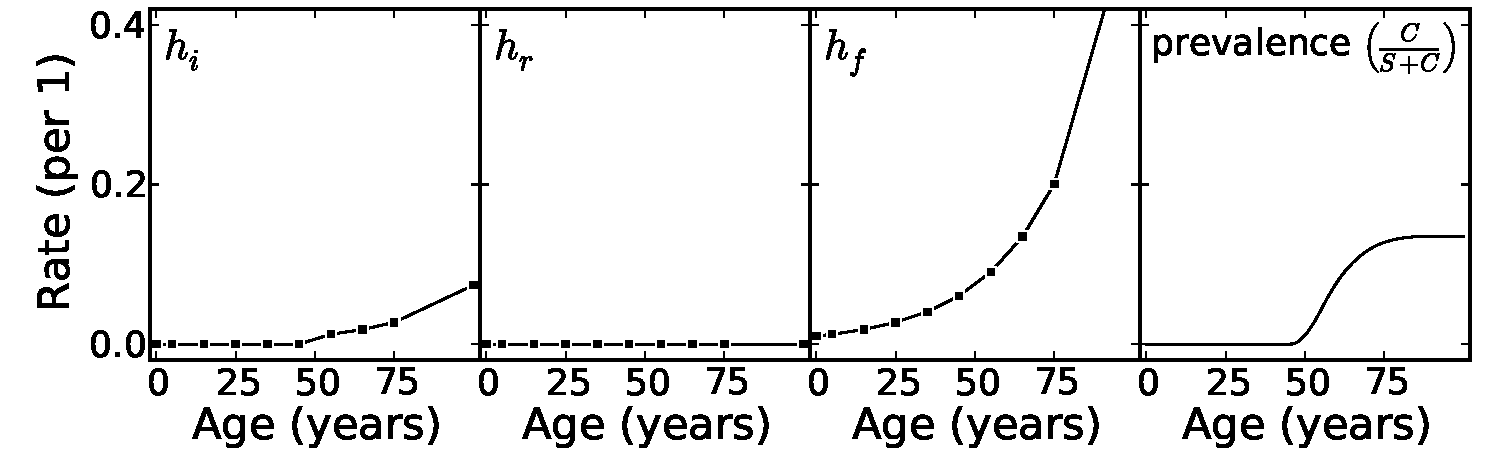
\includegraphics[width=\textwidth]{forward-sim-old_age.png}

And for a disorder related to the reproductive system, like TK, with
substantial excess mortality and incidence during ages 15-60, and
remission that increases substantially at age 55, the consistent age
patterns could look like the following: 

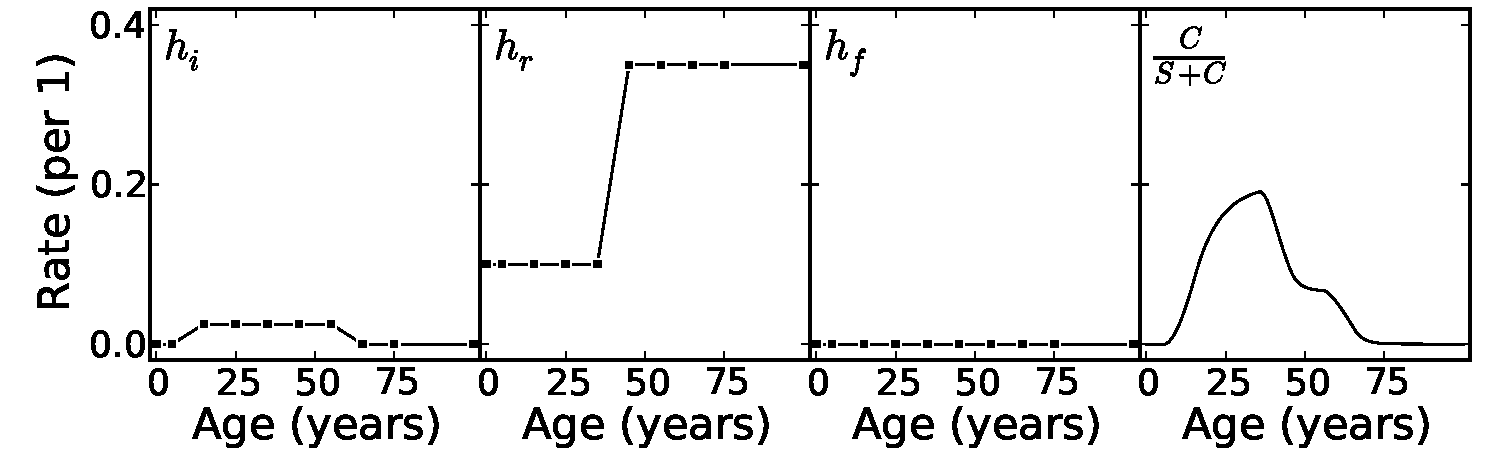
\includegraphics[width=\textwidth]{forward-sim-reproductive.png}

To conclude this series of plots, I've included an "incidence impulse
response" example, showing the prevalence produced to be consistent
with an incidence pattern that is only nonzero for a single age group:

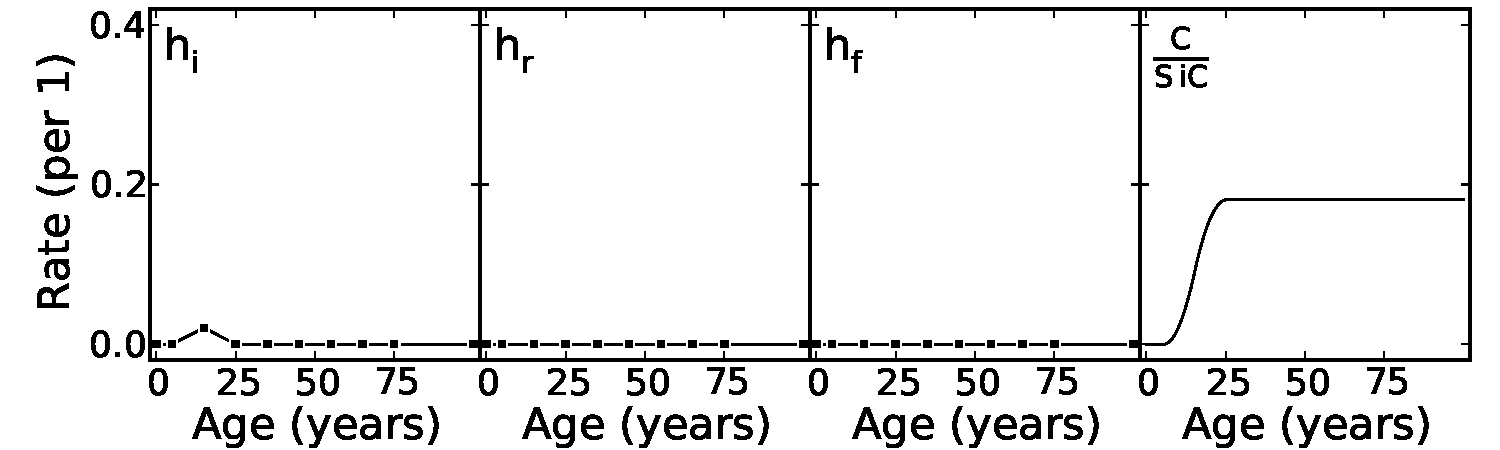
\includegraphics[width=\textwidth]{forward-sim-incidence_pulse.png}

This also provides a mechanism to investigate how wrong the estimates
may become when the assumption that rates are constant over time (for
a given age) is violated. This is the core of my simulation approach
to model validation, to which I will return in section TK.

TK The simulation study approach can be described in full detail here
as well, and can serve as justification for decisions described in the
next two chapters.

\section{What happens to prevalence when the disease incidence or remission or mortality is not constant over time?}

Certain important diseases such as diabetes are widely believed to
have substantial changes in incidence, remission, and mortality rates
over time.  What is the effect of the endemic equilibrium assumption
of the age-specific prevalence. TK plots comparing prevalence from a
synthetic cohort model to a period model using simulation data.
